\subsection{Database}
% \subsubsection{Đặc tả cơ sở dữ liệu}
\begin{figure}[H]
    \centering
    \includegraphics[width=0.95\textwidth]{Images/Design/DB/EERD.png}
    \caption{Sơ đồ cơ sở dữ liệu của hệ thống}
    \label{fig:database-diagram}
\end{figure}

\subsubsection{Các thực thể chính}

\textbf{1. User (cha)} \\[4pt]
Là thực thể gốc của hệ thống, đại diện cho tất cả người dùng (chủ xe, người thuê, quản trị). \\[2pt]
\textbf{Thuộc tính chính:} \texttt{id}, \texttt{fullName}, \texttt{email}, \texttt{phone}, \texttt{avatarUrl}, \texttt{status}, \texttt{role}, \texttt{createdAt}, \texttt{updatedAt}. \\[2pt]
\textbf{Thành phần phức hợp:} \texttt{trustScore \{score, lastCalculated, factors[]\}} dùng để đánh giá độ uy tín của người dùng.

\vspace{6pt}

\textbf{2. Renter} \\[4pt]
Kế thừa từ \texttt{User}, biểu diễn người thuê xe. \\[2pt]
\textbf{Thuộc tính riêng:} \texttt{userId (FK)}, \texttt{address}, \texttt{licenseNum}.

\vspace{6pt}

\textbf{3. Owner} \\[4pt]
Kế thừa từ \texttt{User}, biểu diễn chủ xe. \\[2pt]
\textbf{Thuộc tính riêng:} \texttt{userId (FK)}, \texttt{bankAccount}, \texttt{idCardNum}.

\vspace{6pt}

\textbf{4. Admin} \\[4pt]
Cũng kế thừa từ \texttt{User}, biểu diễn tài khoản quản trị viên hệ thống. \\[2pt]
\textbf{Thuộc tính riêng:} \texttt{userId (FK)}, \texttt{permissions[]} (danh sách quyền thao tác trong hệ thống).

\vspace{6pt}

\textbf{5. Vehicle} \\[4pt]
Đại diện cho xe máy điện được đăng cho thuê bởi \texttt{Owner}. \\[2pt]
\textbf{Thuộc tính chính:} \texttt{id}, \texttt{licensePlate}, \texttt{ownerId (FK)}, \texttt{status}, \texttt{type}, \texttt{model}, \texttt{batteryLevel}, \texttt{pricePerHour}, \texttt{totalRating}, \texttt{totalTrips}, \texttt{imageUrl}, \texttt{createdAt}. \\[2pt]
\textbf{Thành phần phức hợp:} \texttt{location \{latitude, longitude\}} – vị trí hiện tại của xe dùng cho GPS và bản đồ.

\vspace{6pt}

\textbf{6. Booking} \\[4pt]
Biểu diễn giao dịch thuê xe giữa \texttt{Renter} và \texttt{Owner}. \\[2pt]
\textbf{Thuộc tính chính:} \texttt{id}, \texttt{renterId (FK)}, \texttt{vehicleId (FK)}, \texttt{startTime}, \texttt{endTime}, \texttt{actualEndTime}, \texttt{status}, \texttt{totalCost}, \texttt{startLocation}, \texttt{endLocation}, \texttt{createdAt}. \\[2pt]
$\rightarrow$ Dùng để quản lý quy trình thuê xe, tính chi phí, và kiểm soát thời gian.

\vspace{6pt}

\textbf{7. Payment} \\[4pt]
Thực thể lưu thông tin các giao dịch thanh toán liên quan đến \texttt{Booking}. \\[2pt]
\textbf{Thuộc tính chính:} \texttt{id}, \texttt{bookingId (FK)}, \texttt{transactionId}, \texttt{amount}, \texttt{method}, \texttt{status}, \texttt{processedAt}. \\[2pt]
$\rightarrow$ Cho phép quản lý nhiều giao dịch cho cùng một đơn thuê (đặt cọc, thanh toán, hoàn tiền).

\vspace{6pt}

\textbf{8. Review} \\[4pt]
Đại diện cho đánh giá người thuê dành cho xe hoặc chủ xe sau khi kết thúc \texttt{Booking}. \\[2pt]
\textbf{Thuộc tính chính:} \texttt{id}, \texttt{bookingId (FK)}, \texttt{rating}, \texttt{comment}, \texttt{isPending}, \texttt{createdAt}. \\[2pt]
$\rightarrow$ Mỗi \texttt{Booking} có đúng một \texttt{Review} (1:1), giúp tính \texttt{totalRating} cho xe.

\vspace{6pt}

\textbf{9. Notification} \\[4pt]
Dùng để gửi thông báo hệ thống đến người dùng. \\[2pt]
\textbf{Thuộc tính chính:} \texttt{id}, \texttt{userId (FK)}, \texttt{type}, \texttt{title}, \texttt{message}, \texttt{data (JSON)}, \texttt{isRead}, \texttt{sentAt}. \\[2pt]
$\rightarrow$ Hỗ trợ gửi thông báo real-time về trạng thái xe, thanh toán hoặc cảnh báo.

\vspace{6pt}

\textbf{10. AnalyticsReport} \\[4pt]
Được tạo bởi \texttt{Admin} nhằm tổng hợp dữ liệu hoạt động của hệ thống. \\[2pt]
\textbf{Thuộc tính chính:} \texttt{id}, \texttt{adminId (FK)}, \texttt{startDate}, \texttt{endDate}, \texttt{totalRevenue}, \texttt{totalBookings}, \texttt{totalIssues}, \texttt{vehicleDistribution (JSON)}, \texttt{createdAt}. \\[2pt]
$\rightarrow$ Dùng cho mục đích phân tích, báo cáo doanh thu và vận hành.

\subsubsection{Quan hệ giữa các thực thể}

\textbf{1. User -- Notification (1:N)} \\[4pt]
Mỗi \texttt{Notification} phải thuộc về đúng một \texttt{User} (tham gia bắt buộc). 
Một \texttt{User} có thể có không hoặc nhiều thông báo (0..N). 
Triển khai bằng foreign key \texttt{userId} trong bảng \texttt{Notification} với constraint NOT NULL.

\begin{figure}[H]
    \centering
    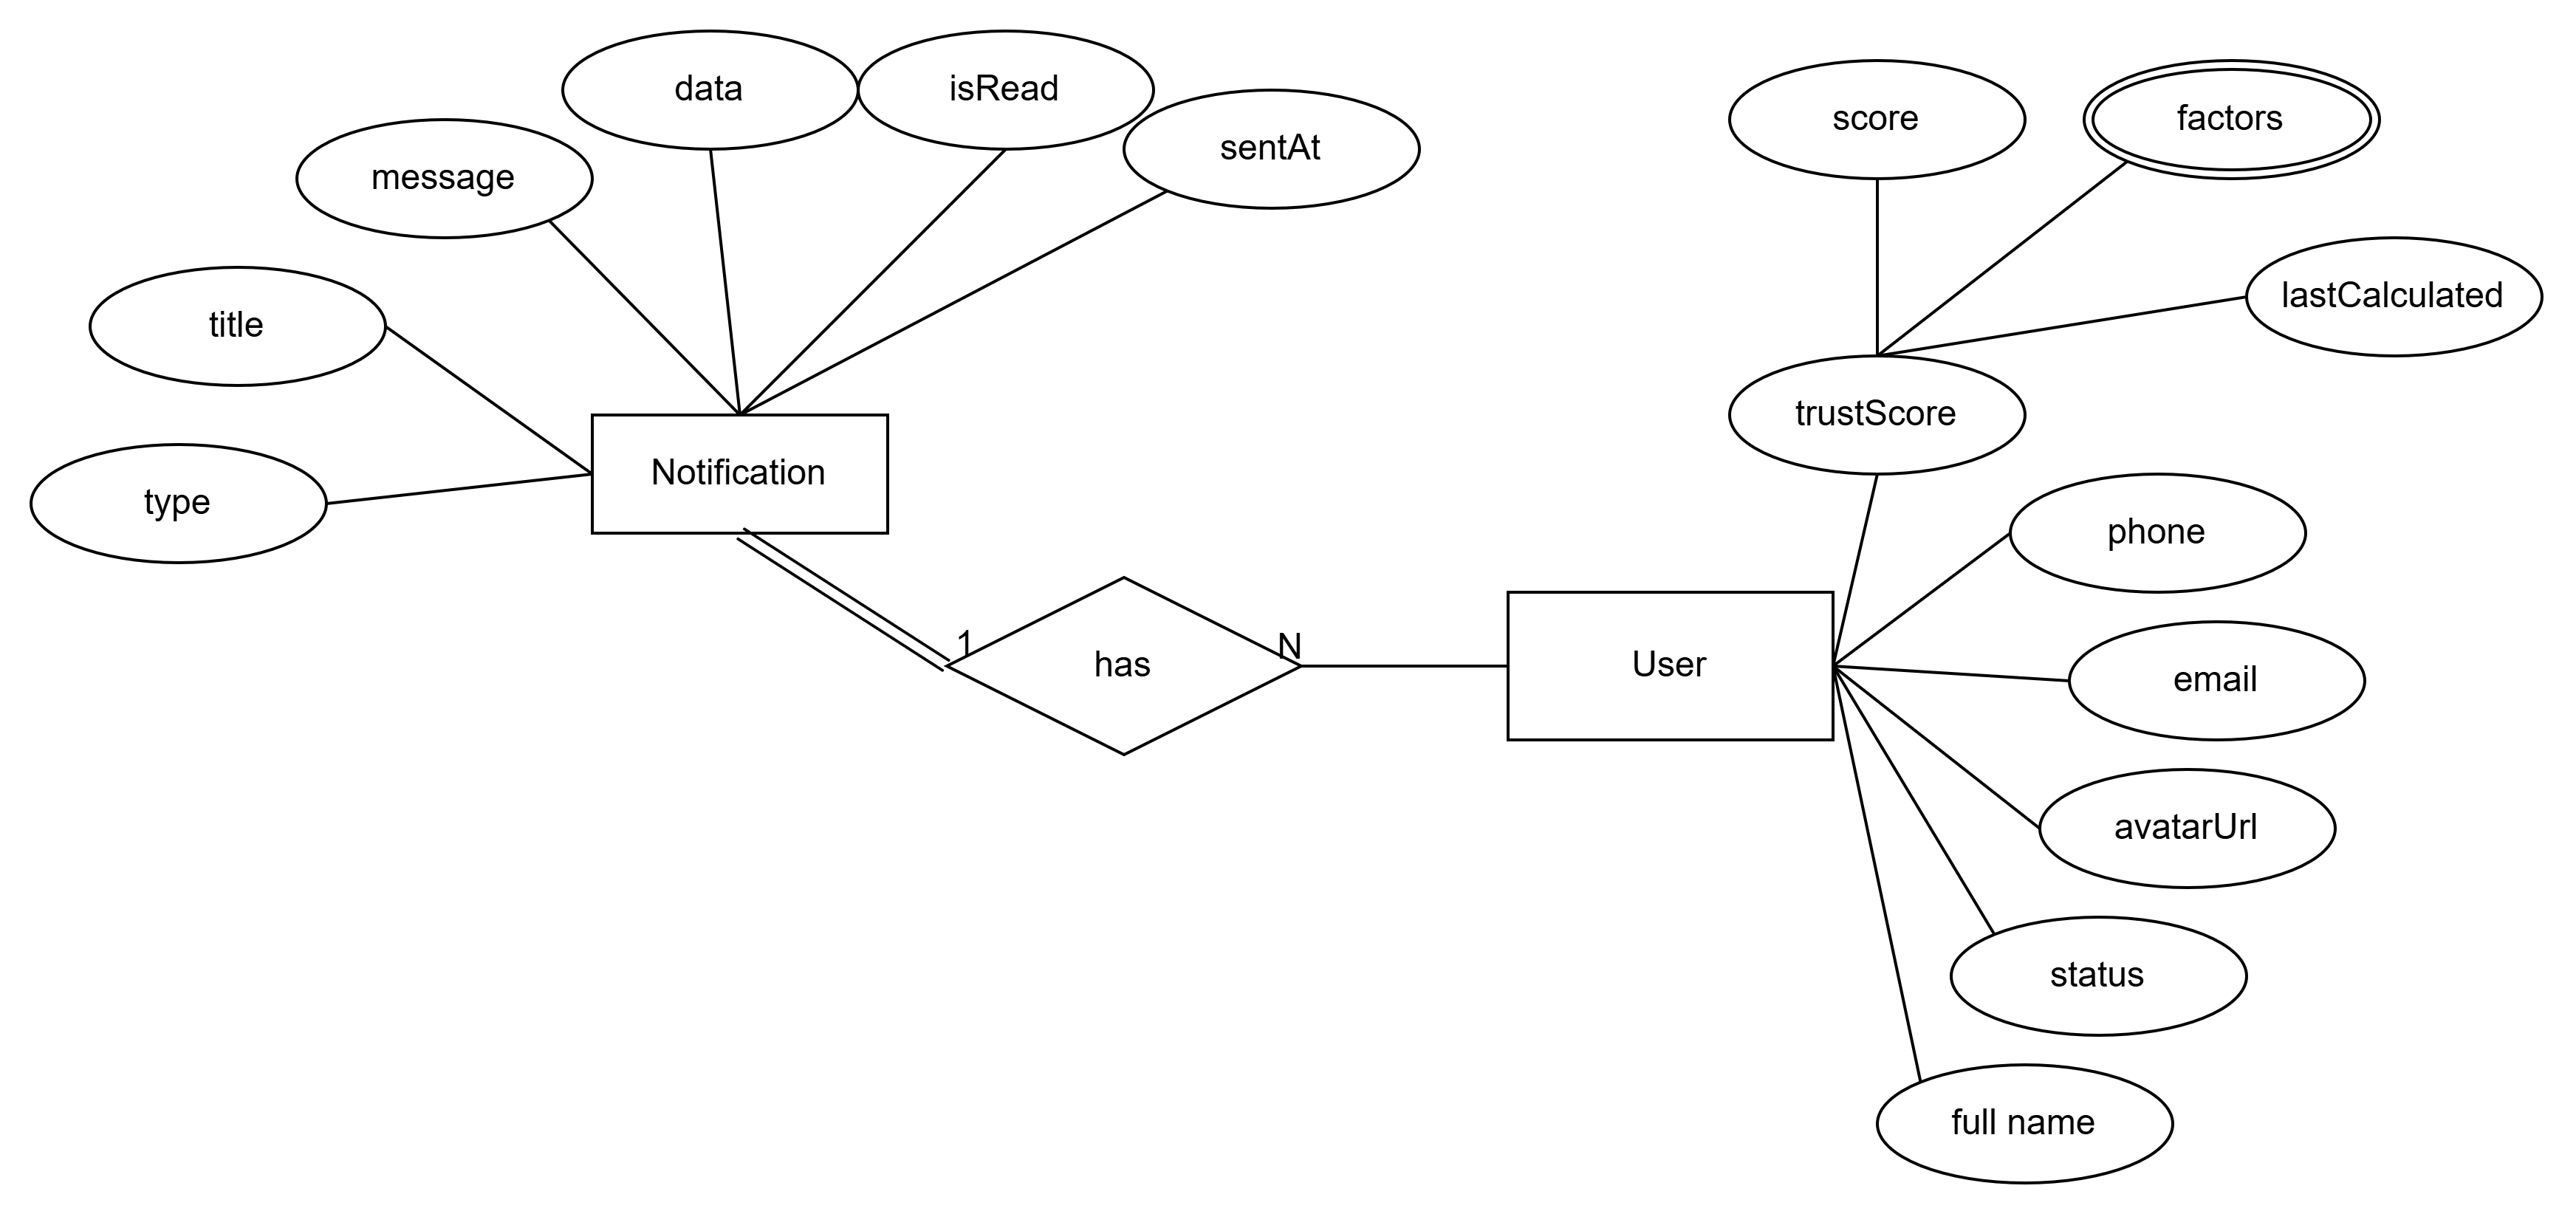
\includegraphics[width=0.5\textwidth]{Images/Design/DB/user-notify.png}
    \caption{Quan hệ giữa \texttt{User} và \texttt{Notification} (1:N)}
    \label{fig:rel-user-notification}
\end{figure}

\vspace{10pt}

\textbf{2. Admin -- AnalyticsReport (1:N)} \\[4pt]
Mỗi \texttt{AnalyticsReport} được tạo bởi đúng một \texttt{Admin} (tham gia bắt buộc). 
Một \texttt{Admin} có thể tạo nhiều báo cáo hoặc chưa tạo báo cáo nào (0..N). 
Foreign key \texttt{adminId} trong bảng \texttt{AnalyticsReport}.

\begin{figure}[H]
    \centering
    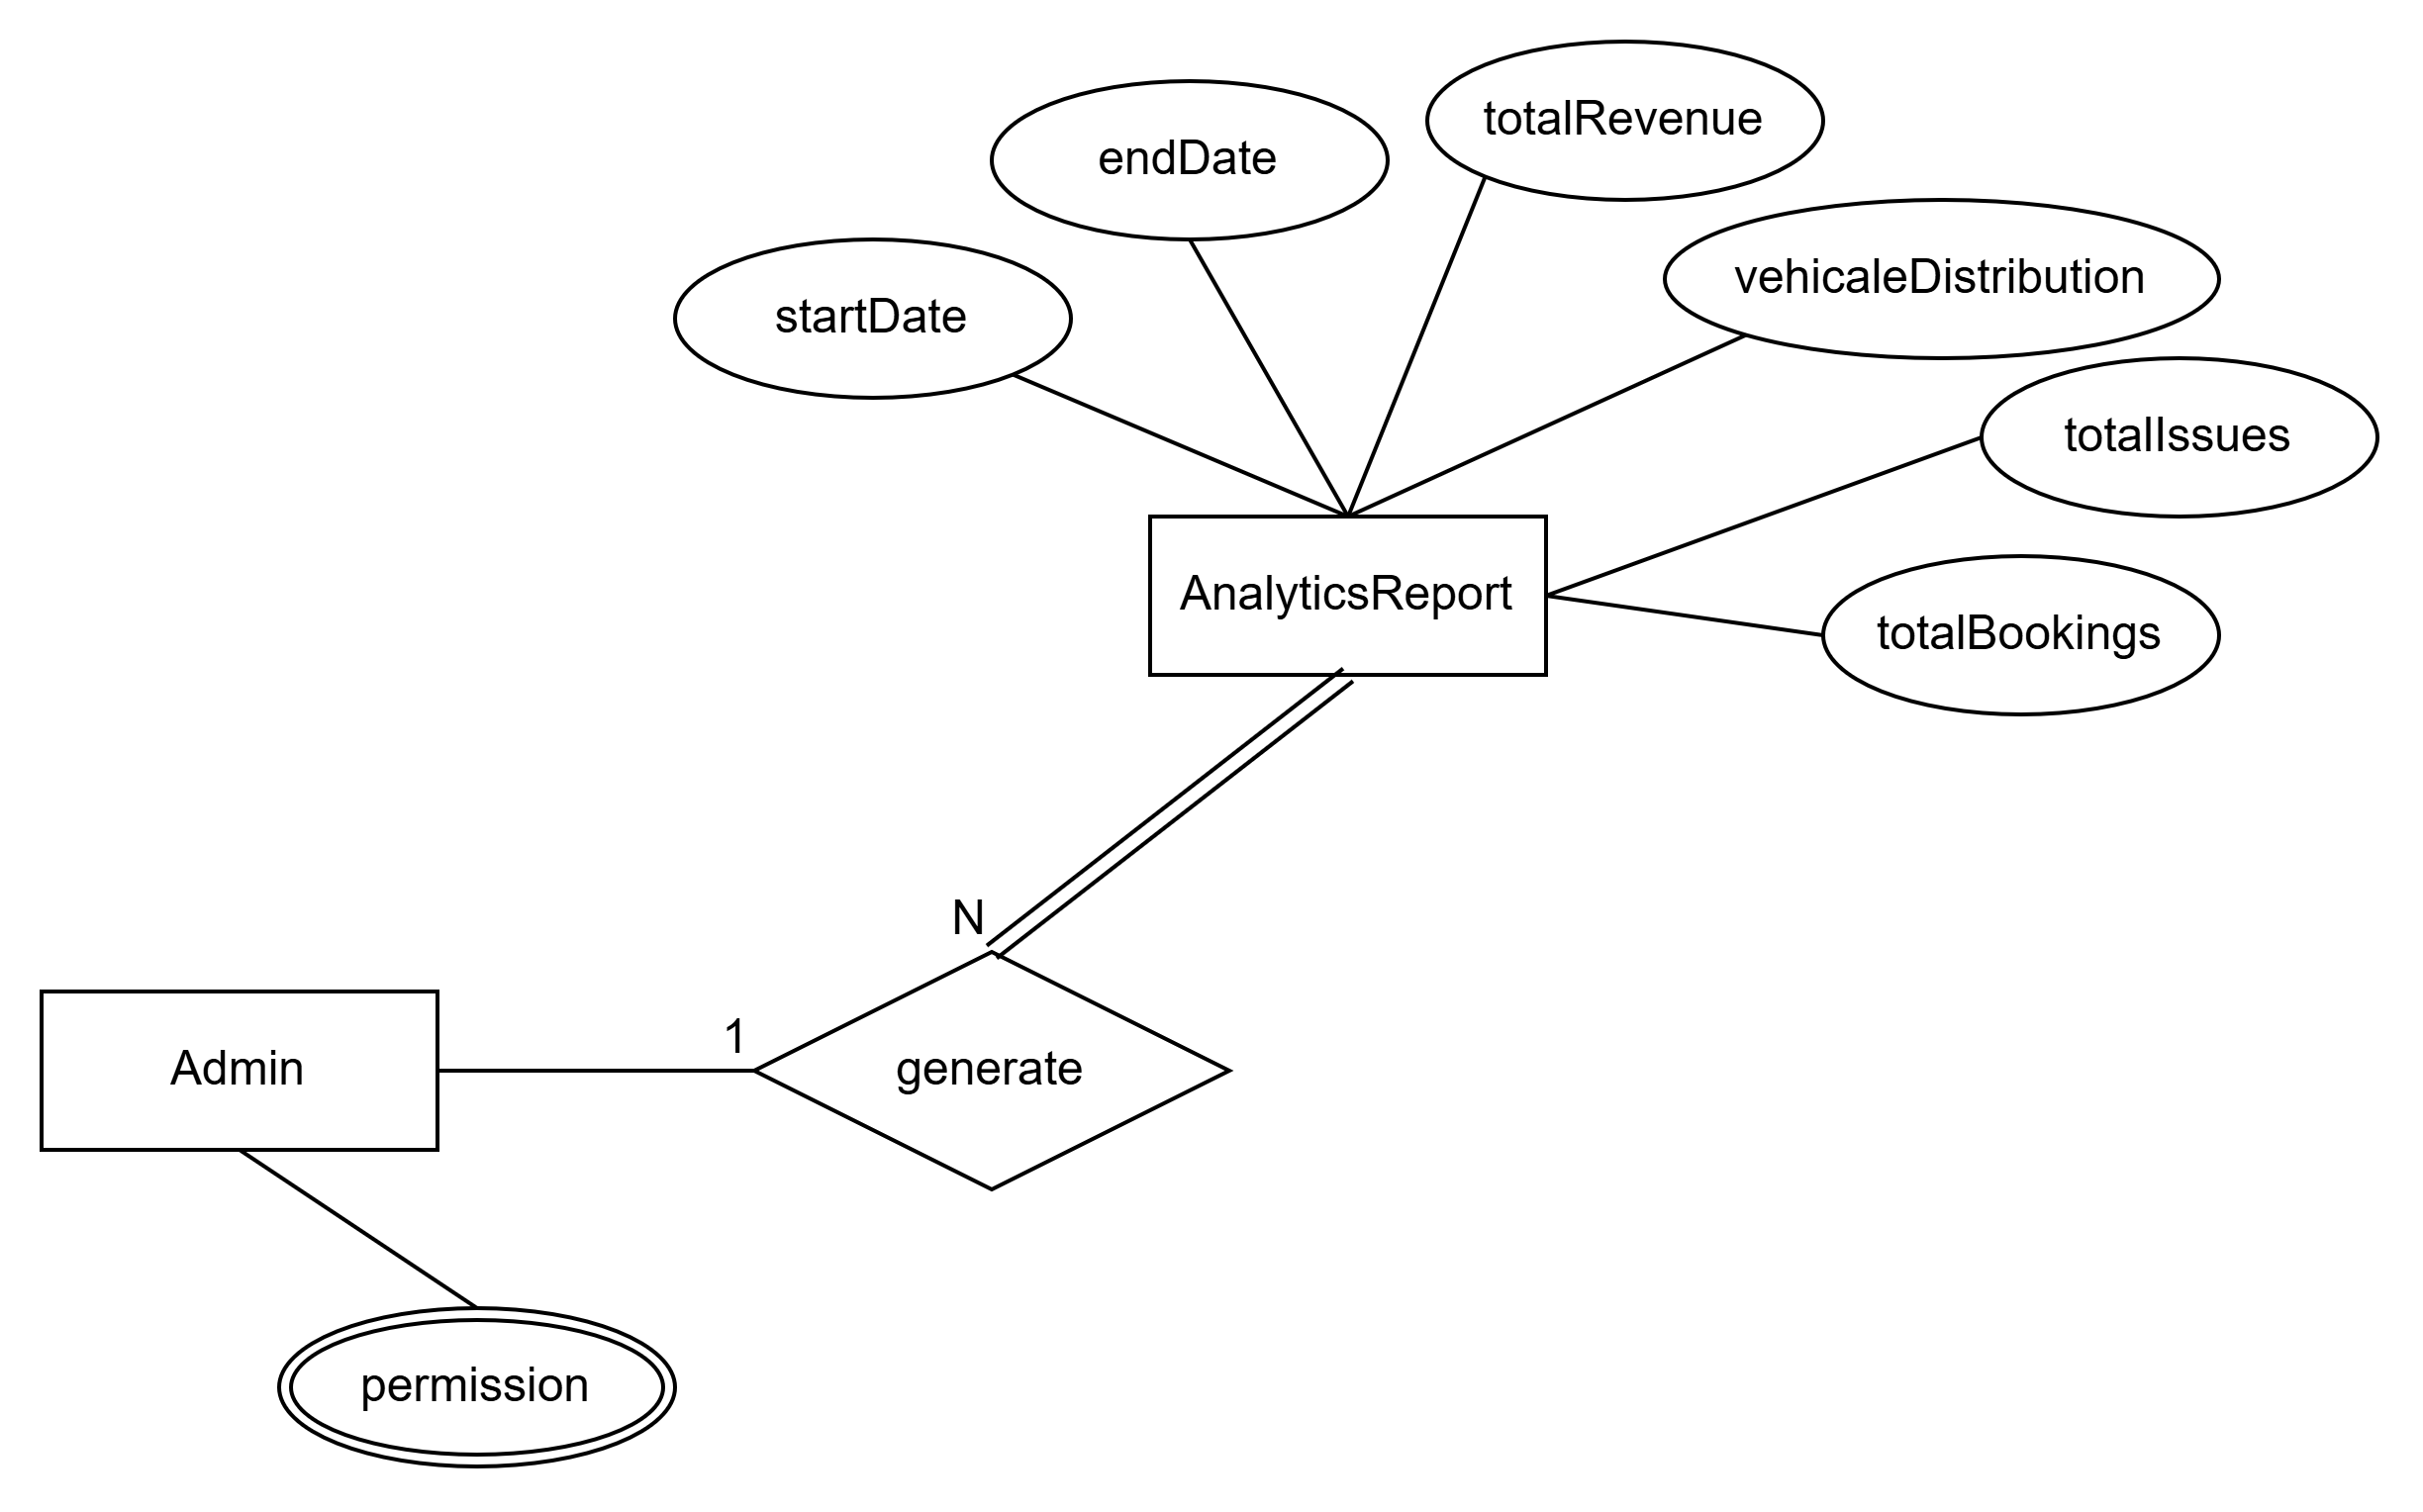
\includegraphics[width=0.5\textwidth]{Images/Design/DB/admin-report.png}
    \caption{Quan hệ giữa \texttt{Admin} và \texttt{AnalyticsReport} (1:N)}
    \label{fig:rel-admin-report}
\end{figure}

\vspace{10pt}

\textbf{3. Owner -- Vehicle (1:N)} \\[4pt]
Mỗi \texttt{Vehicle} phải thuộc về đúng một \texttt{Owner} (tham gia bắt buộc). 
Một \texttt{Owner} có thể sở hữu nhiều xe hoặc chưa có xe nào (0..N). 
Foreign key \texttt{ownerId} trong bảng \texttt{Vehicle} với constraint NOT NULL.

\begin{figure}[H]
    \centering
    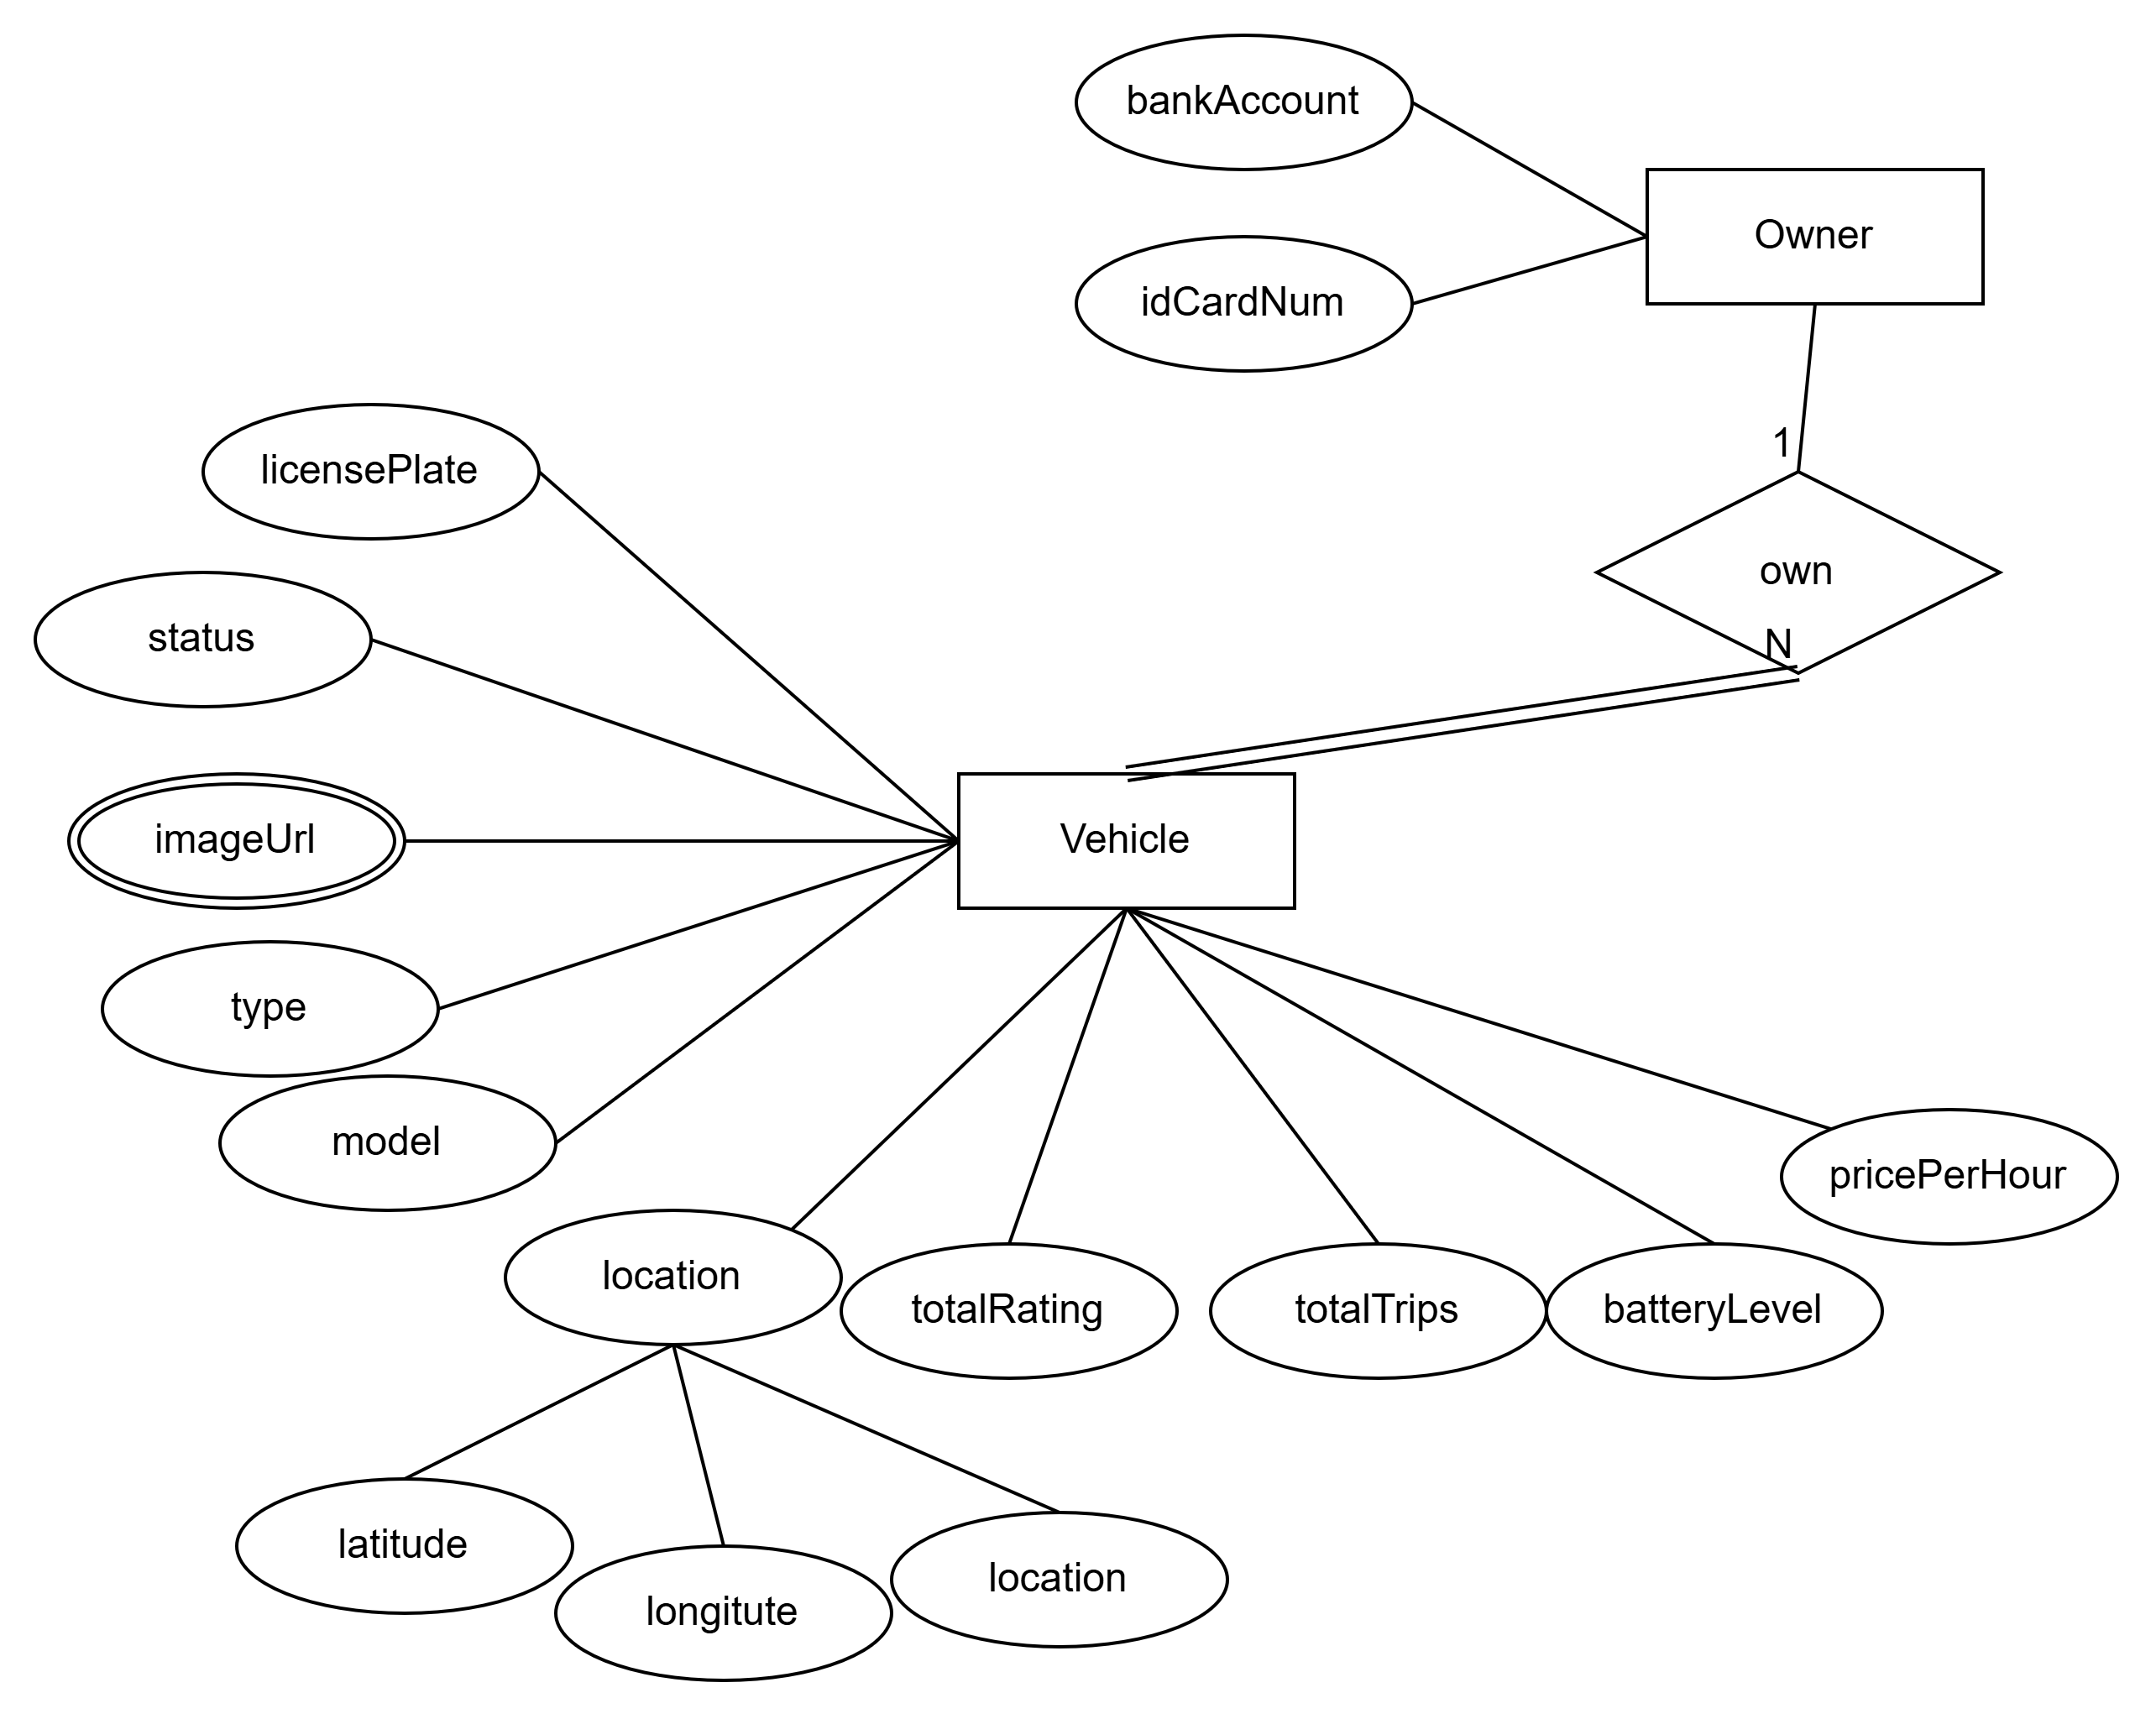
\includegraphics[width=0.5\textwidth]{Images/Design/DB/owner-vehicle.png}
    \caption{Quan hệ giữa \texttt{Owner} và \texttt{Vehicle} (1:N)}
    \label{fig:rel-owner-vehicle}
\end{figure}

\vspace{10pt}

\textbf{4. Renter -- Booking (1:N)} \\[4pt]
Mỗi \texttt{Booking} được tạo bởi đúng một \texttt{Renter} (tham gia bắt buộc). 
Một \texttt{Renter} có thể tạo nhiều booking hoặc chưa có booking nào (0..N). 
Foreign key \texttt{renterId} trong bảng \texttt{Booking} với constraint NOT NULL.

\begin{figure}[H]
    \centering
    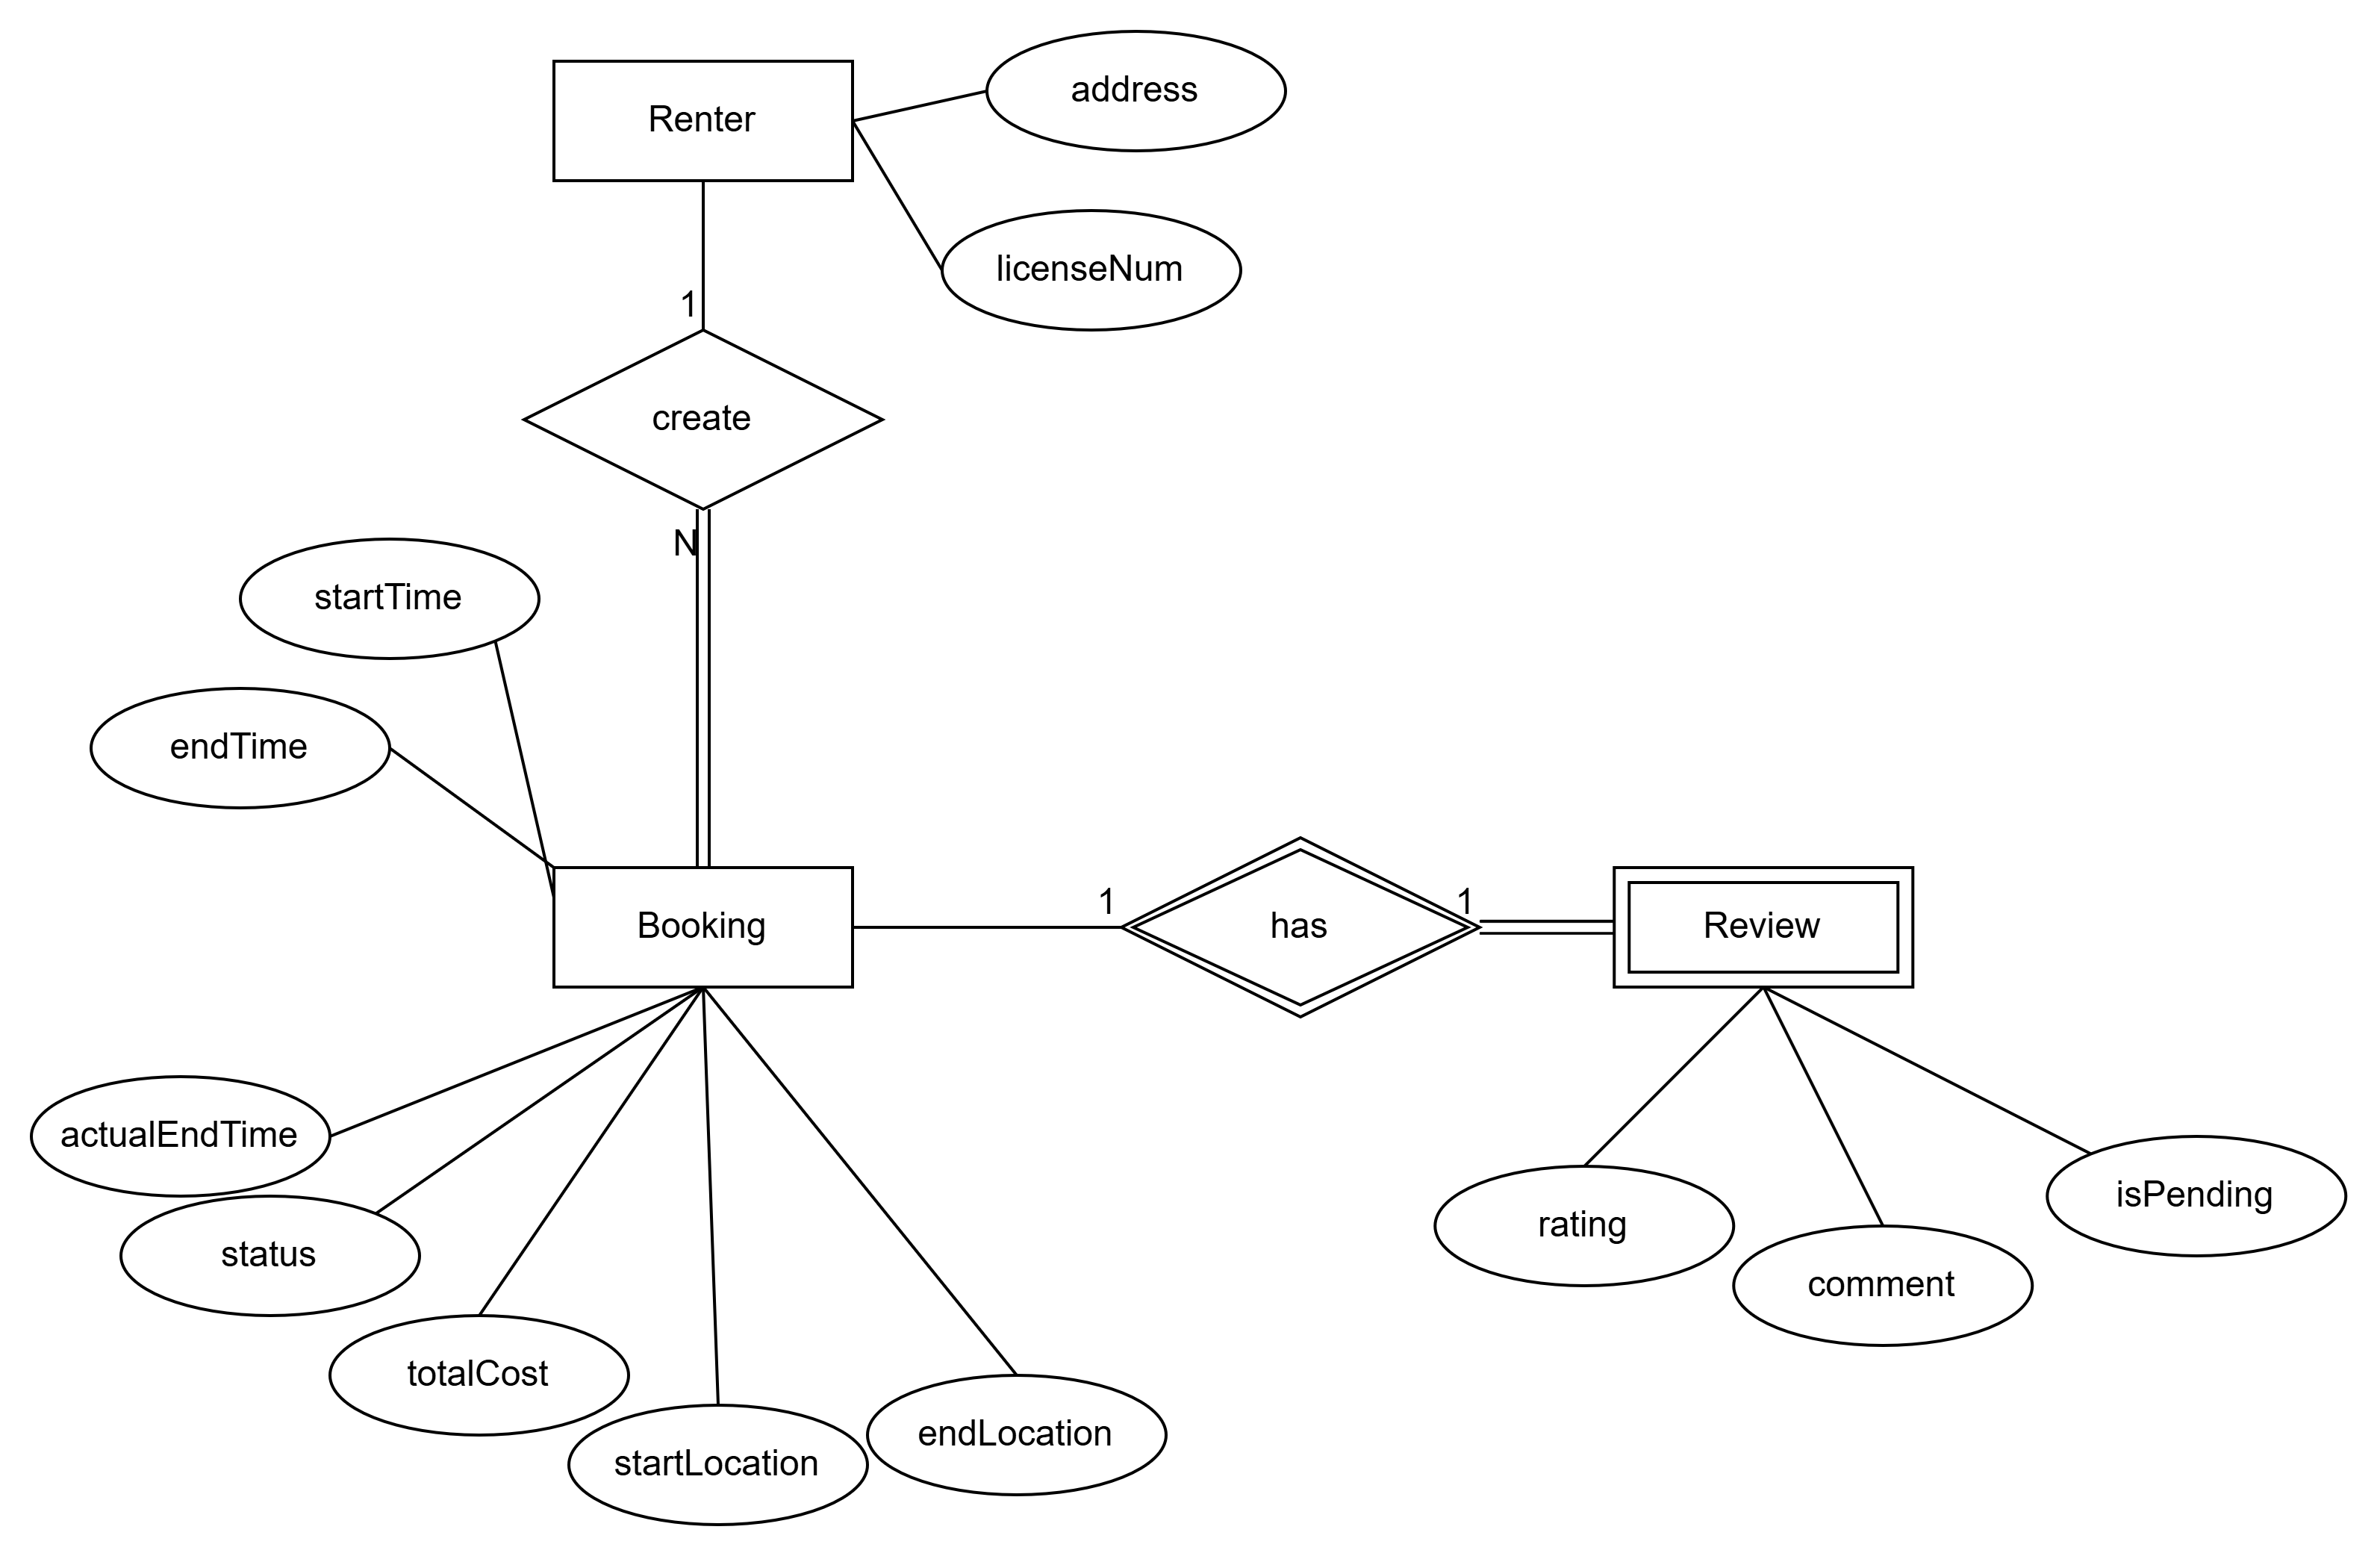
\includegraphics[width=0.5\textwidth]{Images/Design/DB/renter-booking.png}
    \caption{Quan hệ giữa \texttt{Renter} và \texttt{Booking} (1:N)}
    \label{fig:rel-renter-booking}
\end{figure}

\vspace{10pt}

\textbf{5. Booking -- Review (1:1)} \\[4pt]
Mỗi \texttt{Review} phải gắn với đúng một \texttt{Booking} (tham gia bắt buộc). 
Mỗi \texttt{Booking} có đúng một \texttt{Review} (tham gia bắt buộc, quan hệ 1:1). 
Foreign key \texttt{bookingId} trong bảng \texttt{Review} với constraint NOT NULL và UNIQUE để đảm bảo mỗi booking chỉ có một đánh giá.

\textbf{6. Vehicle -- Booking (1:N)} \\[4pt]
Mỗi \texttt{Booking} phải gắn với đúng một \texttt{Vehicle} (tham gia bắt buộc). 
Một \texttt{Vehicle} có thể có nhiều booking hoặc chưa được thuê (0..N). 
Foreign key \texttt{vehicleId} trong bảng \texttt{Booking} với constraint NOT NULL. 
Hỗ trợ kiểm tra xung đột thời gian thuê xe.

\begin{figure}[H]
    \centering
    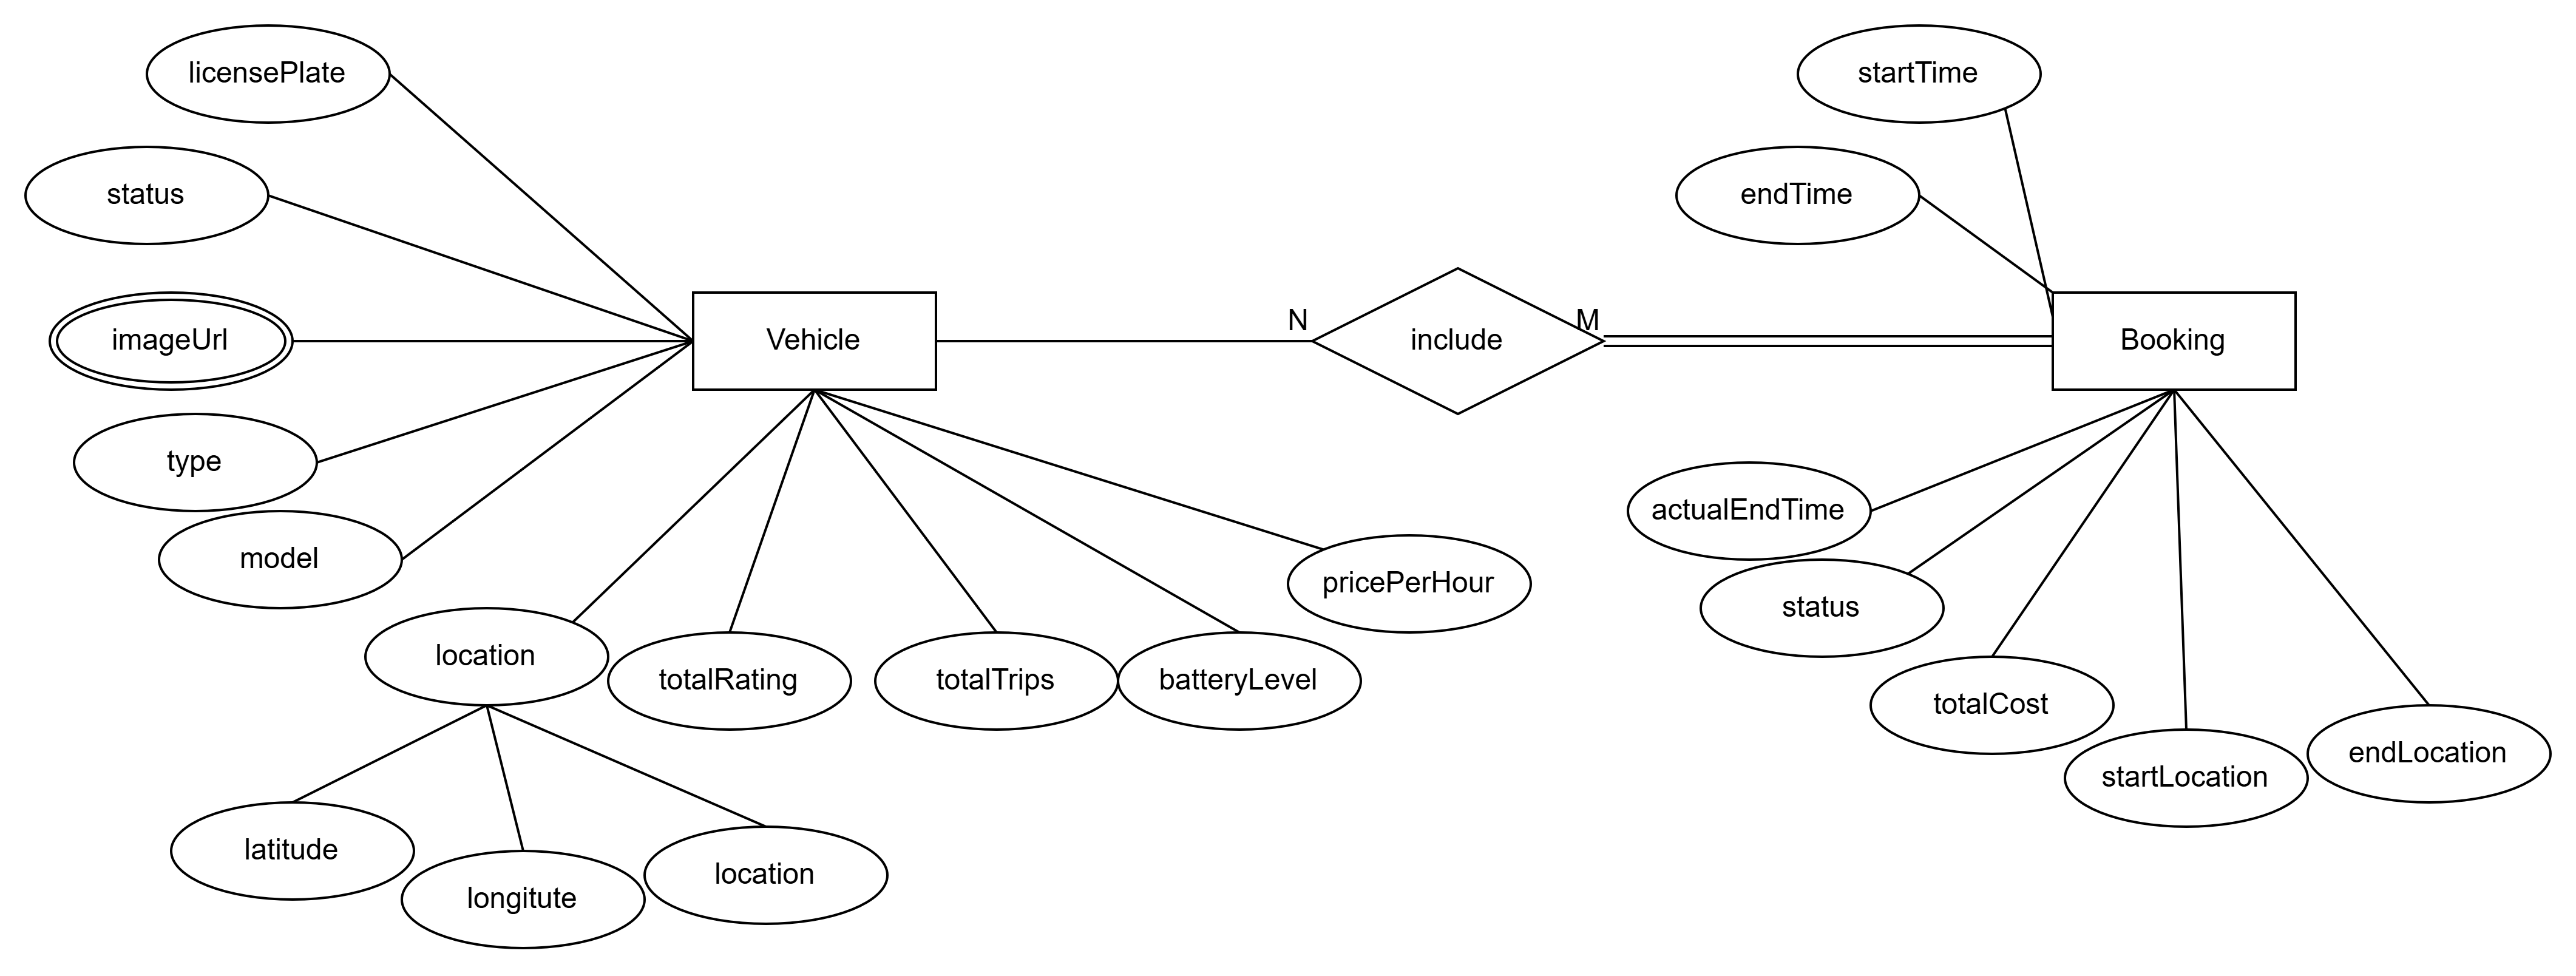
\includegraphics[width=0.5\textwidth]{Images/Design/DB/vehicle-booking.png}
    \caption{Quan hệ giữa \texttt{Vehicle} và \texttt{Booking} (1:N)}
    \label{fig:rel-vehicle-booking}
\end{figure}

\vspace{10pt}

\textbf{7. Booking -- Payment (1:N)} \\[4pt]
Mỗi \texttt{Payment} phải liên kết đến đúng một \texttt{Booking} (tham gia bắt buộc). 
Một \texttt{Booking} có thể có nhiều giao dịch thanh toán (0..N) để xử lý các trường hợp: đặt cọc, thanh toán cuối, hoàn tiền, phạt. 
Foreign key \texttt{bookingId} trong bảng \texttt{Payment}.

\begin{figure}[H]
    \centering
    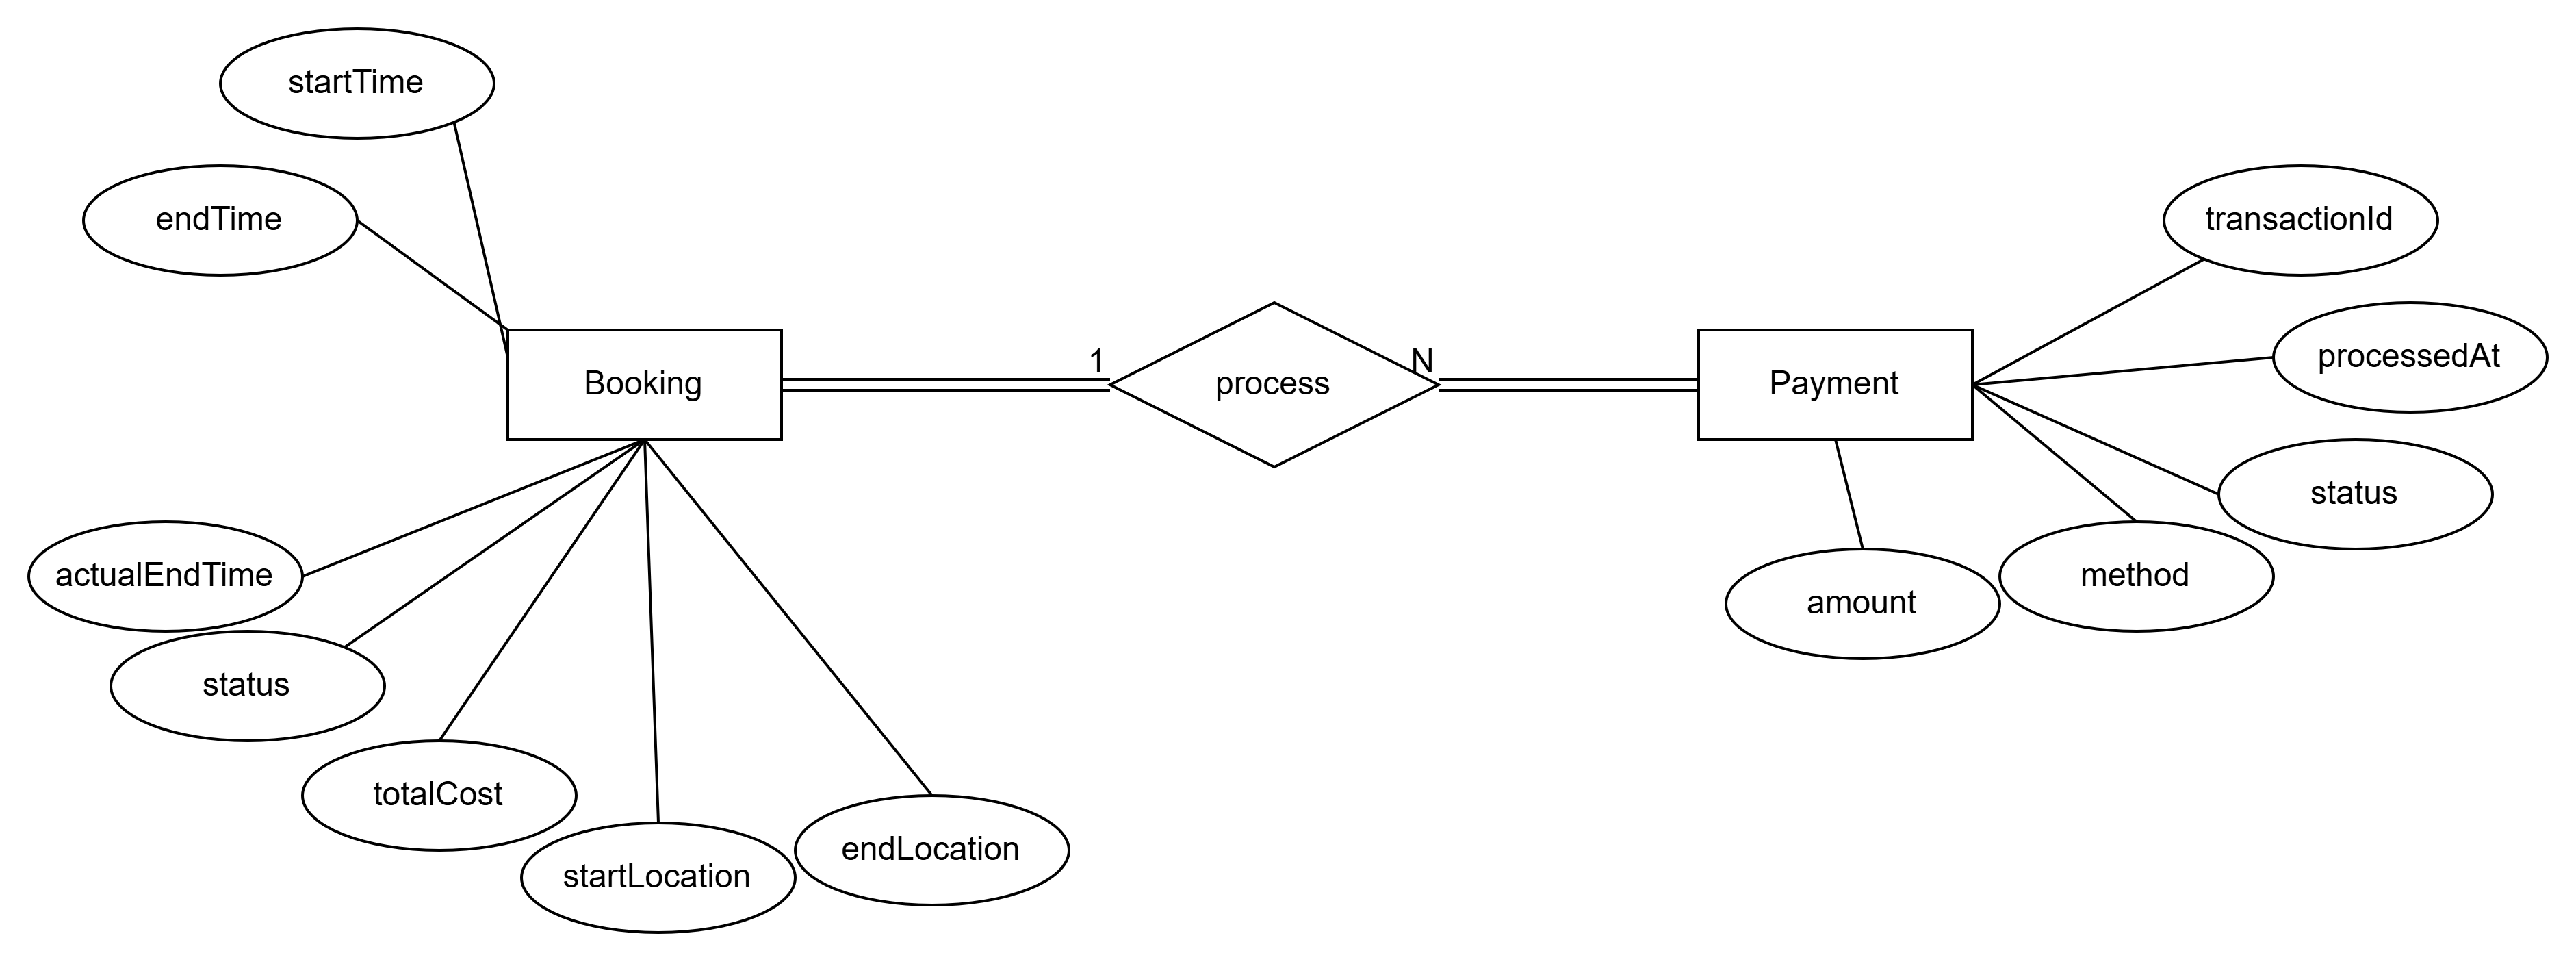
\includegraphics[width=0.5\textwidth]{Images/Design/DB/booking-payment.png}
    \caption{Quan hệ giữa \texttt{Booking} và \texttt{Payment} (1:N)}
    \label{fig:rel-booking-payment}
\end{figure}

\vspace{10pt}

\textbf{8. Mối quan hệ kế thừa giữa các thực thể người dùng hệ thống} \\[4pt]
Mỗi \texttt{User} phải thuộc \textbf{đúng 1} trong 3 loại: \texttt{Renter}, \texttt{Owner}, hoặc \texttt{Admin}.
\texttt{Renter}, \texttt{Owner}, \texttt{Admin} chia sẻ \texttt{userId} (FK → User.id)

\begin{figure}[H]
    \centering
    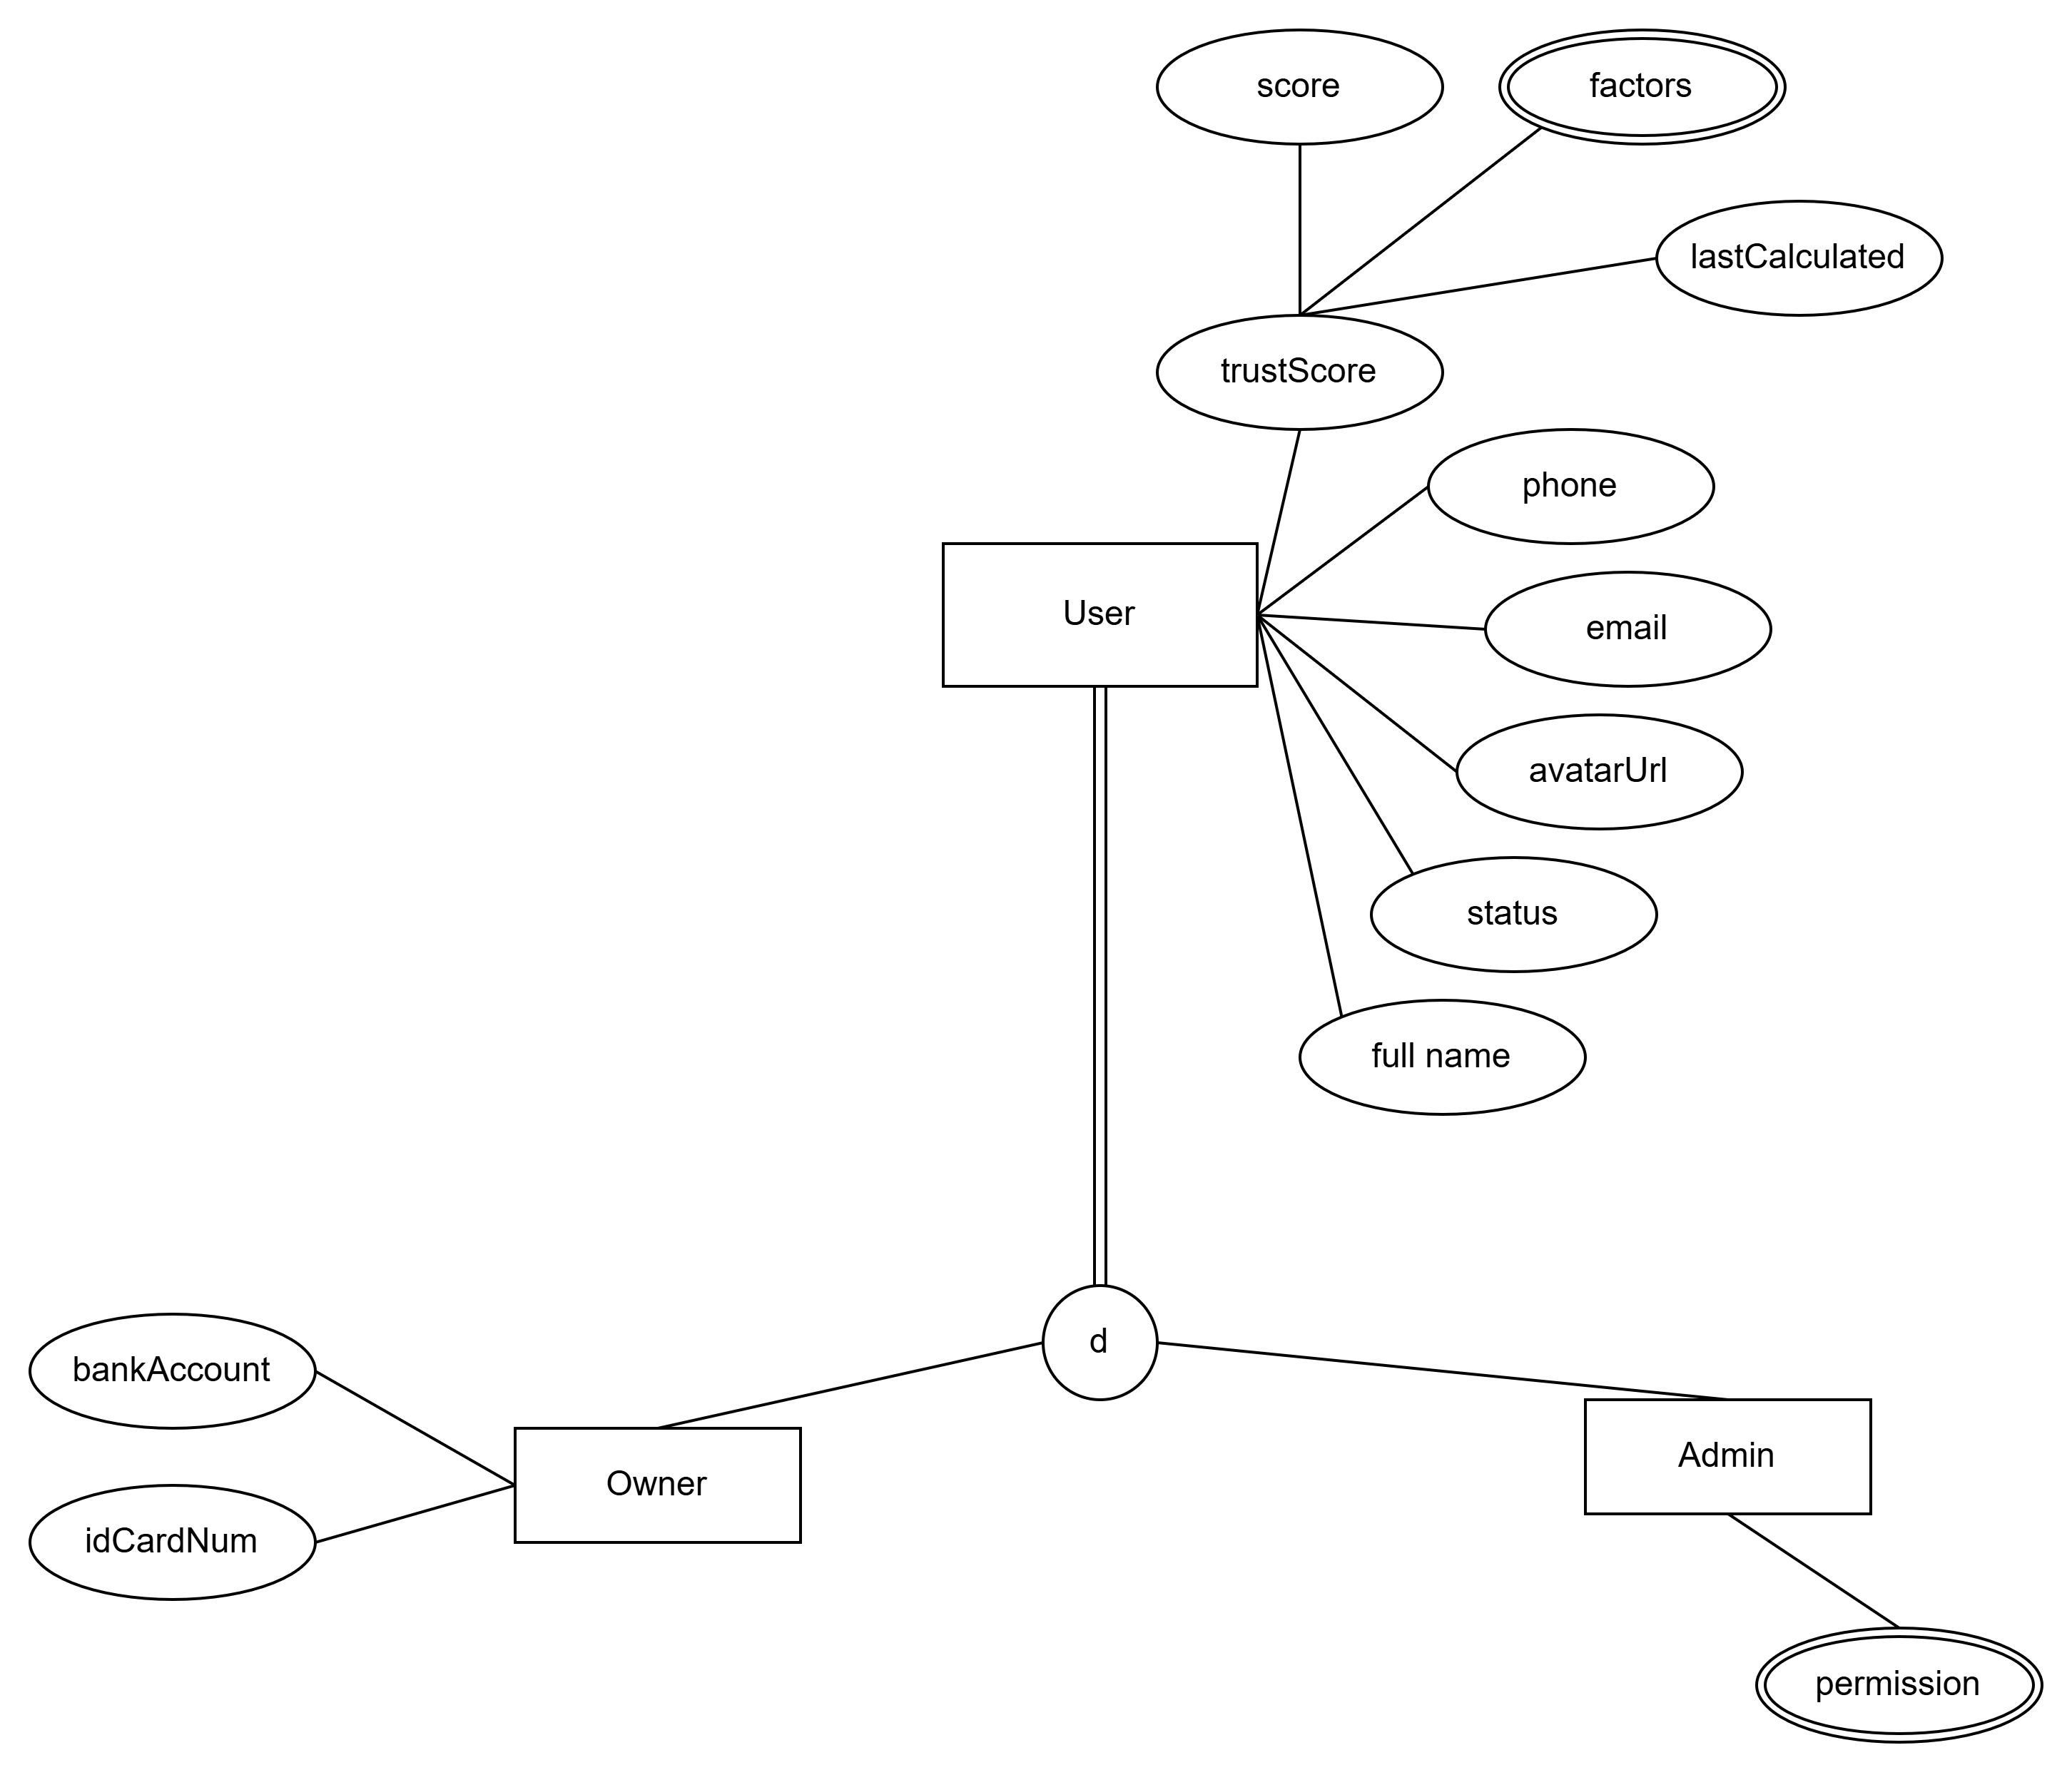
\includegraphics[width=0.5\textwidth]{Images/Design/DB/user.png}
    \caption{Quan hệ kế thừa giữa User với Renter, User, Admin}
    \label{fig:rel-inheritance}
\end{figure}

% \subsubsection*{Kế thừa (Inheritance)}

% Hệ thống sử dụng \textbf{discrete, mandatory inheritance}:
% \begin{itemize}[leftmargin=*]
%     \item Mỗi \texttt{User} phải thuộc \textbf{đúng 1} trong 3 loại: \texttt{Renter}, \texttt{Owner}, hoặc \texttt{Admin}
%     \item Triển khai: Table Per Concrete Class hoặc Single Table Inheritance với trường \texttt{role}
%     \item \texttt{Renter}, \texttt{Owner}, \texttt{Admin} chia sẻ \texttt{userId} (FK → User.id)
% \end{itemize}

% \subsubsection{Ràng buộc toàn vẹn}

% \begin{enumerate}[leftmargin=*]
%     \item \textbf{Notification}: Mỗi notification phải liên kết đến đúng 1 user (NOT NULL \texttt{userId})
%     \item \textbf{Vehicle ownership}: Mỗi vehicle phải có owner (NOT NULL \texttt{ownerId})
%     \item \textbf{Booking}: Mỗi booking phải có renter và vehicle (NOT NULL \texttt{renterId}, \texttt{vehicleId})
%     \item \textbf{Payment}: Mỗi payment phải gắn với 1 booking (NOT NULL \texttt{bookingId})
%     \item \textbf{Review}: Mỗi review phải gắn với 1 booking (NOT NULL \texttt{bookingId}, UNIQUE constraint)
%     \item \textbf{User role}: Mỗi user phải có \texttt{role} $\in$ \{renter, owner, admin\}
%     \item \textbf{Vehicle location}: \texttt{latitude} $\in$ [-90, 90], \texttt{longitude} $\in$ [-180, 180]
%     \item \textbf{Trust score}: \texttt{score} $\in$ [0, 100], \texttt{factors} là JSON array
%     \item \textbf{Booking time}: \texttt{startTime} $ \leqq $ \texttt{endTime}, \texttt{actualEndTime} $\geqq$ \texttt{endTime}
%     \item \textbf{Payment amount}: \texttt{amount} > 0
% \end{enumerate}

% \paragraph{Index và tối ưu hóa}

% \begin{itemize}[leftmargin=*]
%     \item \textbf{Spatial index}: \texttt{CREATE INDEX idx\_vehicle\_location ON vehicles USING GIST (location)}
%     \item \textbf{User queries}: Index trên \texttt{email}, \texttt{phone}, \texttt{status}
%     \item \textbf{Booking queries}: Composite index trên \texttt{(renterId, status)}, \texttt{(vehicleId, startTime)}
%     \item \textbf{Payment queries}: Index trên \texttt{bookingId}, \texttt{status}, \texttt{processedAt}
%     \item \textbf{Full-text search}: Index trên \texttt{Vehicle.model}, \texttt{Vehicle.type}
% \end{itemize}
